\section{Technical Approach}
Automatically finding a close-to-optimal placement of the pipeline registers takes consists of two major parts. First, we must back annotate the Chisel node graph with delay information obtained through the VLSI tools. Once we have the delay data for each Chisel node, we then use simulated annealing to place the pipeline registers based on the delay data obtained with the back annotation tool.

\subsection{Chisel Backannotation}
\begin{table*}
	\centering
	\begin{tabular} 
		{ |c | c| }
		\hline
		\textbf{Origianl backend elaborate flow} & \textbf{Backannotation backend elaborate flow} \\
		\hline \hline
		\multicolumn{2}{| c |}{{\bf -} Set the top module} \\
		\multicolumn{2}{| c |}{{\bf -} Generate muxes} \\
		\multicolumn{2}{| c |}{{\bf -} Execute pre-elaborate transforms} \\
		\multicolumn{2}{| c |}{{\bf -} Gather and sort child modules} \\
		\multicolumn{2}{| c |}{{\bf -} Assign clocks and resets} \\
		\multicolumn{2}{| c |}{{\bf -} Infer bit-widths} \\
		\hline
		{\bf -} \emph{Remove type nodes} & {\bf -} \emph{Collect nodes into components} \\ 
		\cline{2-2}
		& {\bf Intermediate-level Chisel graph} \\
		& {\bf - } \emph{Name nodes} \\
		& {\bf - } \emph{Assign signal names} \\
		& {\bf - } \emph{Perform backannotation} \\ 
		\cline{2-2}
		{\bf -} \emph{Collect nodes into components} & {\bf -} \emph{Remove type nodes} \\
		\hline
		\multicolumn{2}{| c |}{{\bf -} Execute transforms} \\
		\multicolumn{2}{| c |}{{\bf -} Trace nodes (assign bindings)} \\
		\multicolumn{2}{| c |}{{\bf -} Name nodes} \\
		\multicolumn{2}{| c |}{{\bf -} Execute analyses} \\		
		\multicolumn{2}{| c |}{{\bf -} Find combinational loops } \\
		\hline
		{\bf Verilog translation} & \\
		{\bf -} \emph{Assign signal names} & \\
		\hline
	\end{tabular}
	\caption{Comparison between the original backend elaborate flow and the backend elaborate flow for backannotation. Note that signal names are assigned to intermediate-level Chisel graph nodes while they are given during Verilog translation in the original backend.}
	\label{fig:backend_flow}
\end{table*}

\subsubsection{Challenges and Approaches} 
\label{sec:challenges}
There are several challenges for Chisel backannotation. The first is naming problems, which occurs when the destination nodes have different names. Signal names are given during Verilog translation, a process after the elaborate process and this is highly affected by graph topology. However, other tools like the automatic pipelining tool are expected to manipulate a high-level Chisel graph which goes through only part of the elaborate process, while the Chisel backannotator wants to use a low-level Chisel graph which is elaborated by the backend. The two graphs look different from each other, which makes it difficult to match signal names between them. Thus, we define the intermediate-level Chisel graph so that both the backannotator and the tools are satisfied.

Table \ref{fig:backend_flow} compares the backend elaborate flow for backannotation with the original elaborate flow. \textbf{Remove type nodes} and \textbf{Trace nodes} are processes tools want to avoid because they change the graph topology undesirably. Thus, we apply processes necessary for backannotation to an initial graph prior to \textbf{Remove type nodes} and \textbf{Trace nodes}, and then obtain an intermediate-level Chisel graph. Signal names are assigned to intermediate graph nodes, and backannotation is performed. Tools like the automatic pipelining tool manipulate this backannotated graph.

The second challenge is missing signals during logic synthesis. Missing signals are inevitable although we give signal preserving commands to Synopsys tools. This occurs when Chisel graph nodes are mapped to generic logic blocks by Synopsys tools. These generic logic blocks are replaced by technology-dependent logic cells, and signals of the logics are replaced by arbitrary nets during the compilation of Synopsys tools.

An approach to this problem is calculate the arrival time difference between two non-missing signals in a timing path, and assigning the average value of the difference to missing signals. For example, suppose we have a path from X through T1, T2, and T3 to Y where T1, T2, and T3 are missing signals, and the arrival times of X and Y are 0.1 and 0.5, respectively. The arrival time difference between X and Y is 0.4, and the delays for T1, T2, T3, and Y are estimated as 0.1.

Another challenge is conditional statements like \emph{if} and \emph{switch}. These statements are converted into logic gates during logic synthesis which are not visible in Chisel graphs. Currently, we cannot directly backannotate corresponding nodes in the Chisel graphs with their delays. Instead, there is a separate variable in reset and enable signals of registers. The Chisel backannotator uses this variable to mark the delays of conditional statements.

\subsubsection{Delay Backannotation Flow}
The Chisel backannotator annotates intermediate-level Chisel graph nodes with delay information as follows:

{\bf (1) Finds all possible timing paths}
	
The timing analysis tool finds and analyzes all of the timing paths in the design. The data is launched at the start point of a timing path by a clock edge, propagated through combinational logic in the path, and captured at the endpoint of the path by another clock edge. The startpoint of a path is a clock pin of a sequential element or and an input port of the design. The endpoint is a data input pin of a sequential logic or an output port of the design. 

The Chisel backannotator uses timing path reports to annotate Chisel graphs. It finds all possible timing paths in a Chisel graph to be reported. A timing path is given as a list of Chisel nodes where the start node represents either a register or an input port, the end node represents a register or an output port, and the intermediate nodes represent combinational logics. 

{\bf (2) Generates a tcl script}

A tcl script consists of a set of Synopsys tool commands. For backannotation, it is necessary to generate a customized tcl script to obtain design specific timing path reports. A tcl script generated by the Chisel backannotator contains commands to report timing information of the paths found in Step {\bf (1)}, as well as basic commands to specify libraries, read and compile designs, and write the results. 

{\bf (3) Executes Synopsys tools}

In this step, the Chisel backannotator executes Sysnopsys tools with the tcl script generated by Step {\bf (2)}, which produces timing path reports. Note that the RTL used by Synopsys tools is produced in advance by the first run of the Chisel Verilog backend.

{\bf (4) Reads the timing report and calculates the delays of Chisel nodes}

The timing report produced by Step {\bf (3)} contains 1) the output signals of Chisel nodes (including missing signals) consisting of a timing paths, and 2) the arrival times of nets in the path. The output signal of a Chisel node corresponds to a net in the gate-level netlist, and its arrival time is obtained from the timing report. Thus, the node delay is calculated as the arrival time difference between its output signal and the output signal of its input Chisel graph node.

However, it is impossible to know the arrival times of missing signals because they do not have a corresponding net in the gate netlist. In this step, the chisel backannotator estimates the arrival times of missing signals using the method in Section \ref{sec:challenges}. It also calculates the delays of conditional statements as the arrival time difference between a register and its reset or enable signal.

{\bf (5) Annotates the Chisel graph with the delays}

The Chisel backannotator annotates the intermediate Chisel graph with delays obtained from Step {\bf (4)}.

{\bf (6) Calculates the critical path delay}

In this step, the Chisel backannotator calculates the sum of the Chisel node delays in a timing paths. The critical path is a timing path which has the largest sum. The critical path delay can be used to verify the accuracy of the Chisel backannotator.

\subsection{Automatic Pipeline Register Placement}
The automatic pipelining tool first creates a legal placement of pipeline registers based on the stage numbers of the user annotated nodes and then uses simulated annealing based on the delay data provided by the backannotation to find a close-to-optimal placement of the pipeline registers. 

\subsubsection{Pipeline Legality}
For a pipeline register placement to be legal, it must satisfy the following three conditions:

{\bf (1)} Every combinational logic node has all input signal with the same stage number.  

{\bf (2)} The stage number of every combinational logic node's output signal is greater than or equal to the maximum of its input signal stage numbers. 

{\bf (3)} There are two ways to determine the stage number of a node. One way is to trace through the node's inputs to a pipeline register and set the stage number of the node equal to the stage number of that pipeline register. Another way is to trace through the node’s consumers to a pipeline register and set the stage number of the node equal to the stage number of that pipeline register {\tt >=}  1. For all nodes in the graph, the stage number of the node obtained through both methods must be the same.

\subsubsection{Wire Node Insertion}
\label{wiresection}
Before the automatic pipelining tool infers the initial legal placement of the pipeline registers, it inserts Chisel Bits nodes representing wires between combinational logic nodes in the original design. This ensures that a pipeline boundary never has to fall across a combinational logic node, which would be difficult to reconcile with the notion of Pipeline Legality discussed above.
\subsubsection{Initial Placement}
The automatic pipelining tool breaks cycles in the Chisel graph by splitting architectural registers(registers present in the original one cycle design) into read and write points. The read point consists of the output of the register and the write points consist of the write data and write enables going into the register. Hence, the data sources in the Chisel node graph are read points, input nodes, and constants and the data sinks in the Chisel node are the write points and output node.

Due to reasons that will become apparent from the algorithm discussed below, in general the designer must annotate all of the data sources and data sinks in the Chisel graph in order for the automatic pipelining tool to produce a legal pipeline register placement.

The automatic pipelining tool produces the initial legal pipeline placement by propagating stage numbers out from the user annotated Chisel nodes to their inputs and consumers in a pseudo breadth-first-search (BFS) manner. When two propagation frontiers with different stage numbers meet at the same node, propagation down that path stops and pipeline registers are inserted at that node.

We must maintain the following conditions during the pipeline stage propagation process:

{\bf (1)} Adjust the propagation rates of each propagation frontier so that two different propagation frontiers never meet at a combinational logic node and always meets at a wire node mentioned in \ref{wiresection}, because it does not make sense to split a combinational logic node in half with a pipeline register.

{\bf (2)}  The stage number propagated to a combinational logic node with multiple inputs must be the maximum of the stage numbers of all of its inputs. If this was not maintained, we would have some inputs of the combinational logic node have a greater stage number than the stage number of the output of the combinational node, which violates 2nd condition of Pipeline Legality. This also means that we cannot propagate to a Chisel node with multiple inputs from the input side until all of its inputs have been propagated to.

{\bf (3)} The stage number propagated to a combinational logic node with multiple consumers must be the minimum of the stage numbers of all of its consumers. If this was not maintained, we would have some consumers of the combinational logic node have a smaller stage number than the stage number of the output of the combinational node, which cause that consumer to violate the 3rd condition of Pipeline Legality. This also means that we cannot propagate to a Chisel node with multiple consumers from the consumer side until all of its consumers have been propagated to.

Due to conditions (2) and (3), if not all of the data sources and data sinks are user annotated, the stage propagation process may never complete.
\subsubsection{Optimizing Register Placement}
Once the tool finds an initial legal pipeline register placement, it uses simulated annealing to optimize the placement of the pipeline registers based on the delay data obtained from the Chisel backannotation.

{\bf Simulated Annealing Algorithm}.

We want a fast method of finding a close-to-optimal pipeline register placement without getting stuck at local minimums. Simulated annealing is a gradient decent like algorithm that iteratively improves upon the current solution by randomly generating neighbor solutions from the current solution and then picking the neighboring solution that decreases the cost function the most as the next solution. Unlike gradient decent, simulated annealing occasionally picks neighbor solutions that are worse than the current solution. This allows the algorithm to avoid getting stuck at local minimums. The algorithm uses the following formula to decide if it should choose a neighbor solution as the next solution:
$$
e^{-\Delta cost/T} > R(0,1)
$$

%\begin{figure}[htb]
%\centering
%\resizebox{\columnwidth}{!}{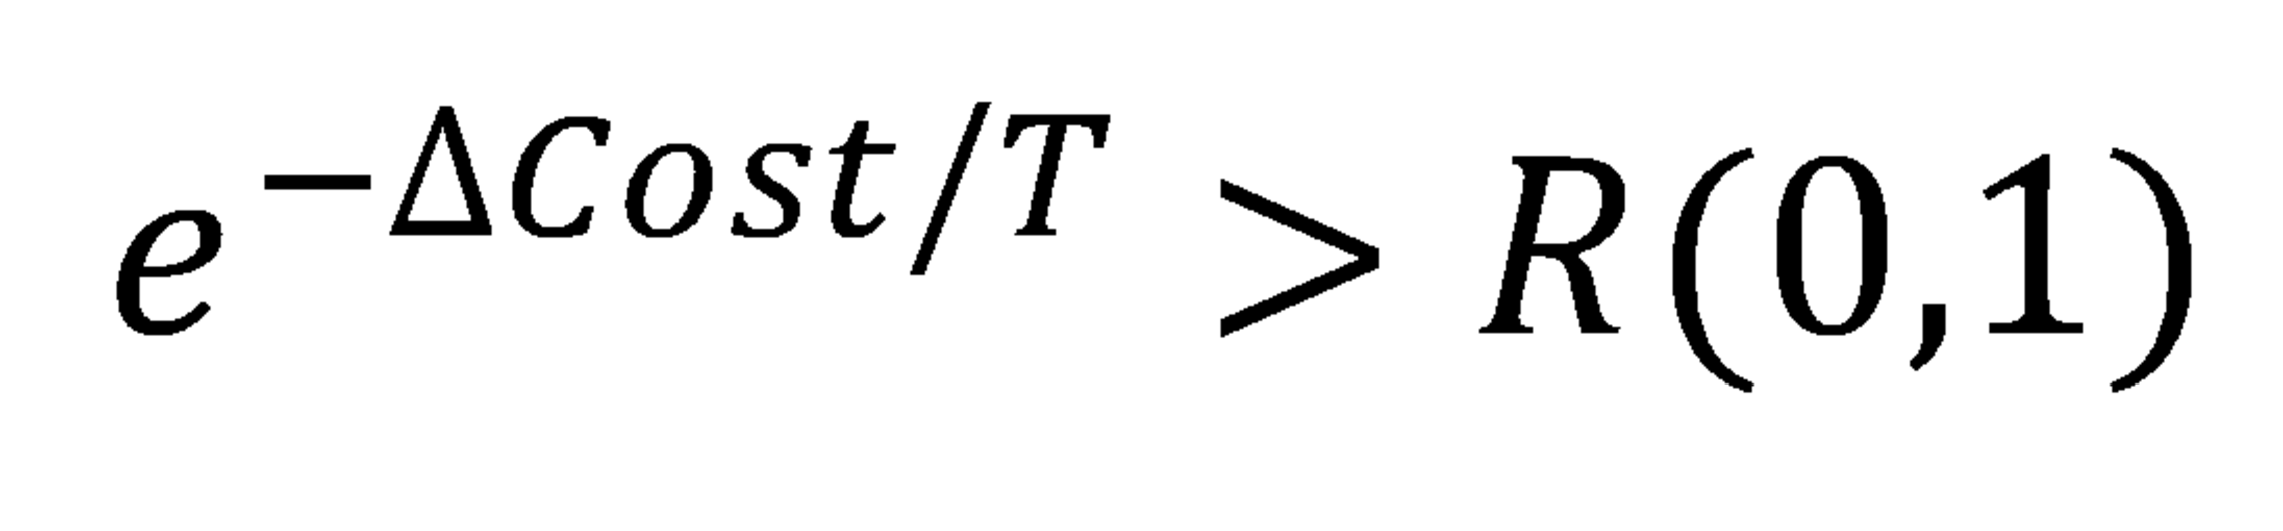
\includegraphics{figures/SimulatedEq.pdf}}
%\end{figure}

$R(0,1)$ is a random number in the interval $[0, 1]$. At higher values of $T$ (temperature), the algorithm is more likely to accept bad solutions. As the algorithm progresses, the value of T is lowered so that the algorithm eventually settles on a close-to-optimal solution. On each iteration, we lower $T$ by $T$ * cooling rate.


This cooling policy forces the algorithm to try many bad solutions in the very early iterations and then focus on trying good solutions for the majority of the remaining iterations. There are many possible cooling schedules, but this one has worked well for us.

We use a starting temperature of 10000 and a cooling rate of 0.002. We terminate the algorithm when the temperature falls below 0.01 or if the iteration count exceeds 3000. We have found the critical path length has generally converged by those two limits in the designs we evaluated.

The cost function used for our problem is the maximum combinational path length in the design and we obtain neighbor solutions from the current solution by moving Chisel nodes across pipeline boundaries in a way that mains a legal pipeline register placement


{\bf Generating Neighbor Solutions}.

We must maintain a legal pipeline register placement as we generate new pipeline register placements from the current pipeline register placement. To accomplish this, we look at the current pipeline register placement and choose eligible combinational logic nodes to move across pipeline stage boundaries. A combinational logic nodes is eligible if it meets the following conditions:

{\bf (1)} 
The node is not an architectural register read point, architectural register write point, input node, or output node. We choose to not allow the automatic pipelining tool to move these nodes because doing so could have large unforeseen performance implications. For example, if we are pipelining a RISC processor, moving the write point of the PC register to later stages will cause branches to be resolved later in the pipeline and thus cause a larger branch mispredict penalty.

{\bf (2)}  
The node outputs directly to a pipeline register. In this case, it is safe to move the node forward across the pipeline boundary by removing the pipeline register from the output of the node and adding pipeline registers to all the inputs of the node and still maintain a legal pipeline register placement. 

{\bf (3)} 
The node has all of its inputs driven directly by a pipeline register. In this case, it is safe to move the node backward across the pipeline boundary by removing the pipeline registers from the inputs of the node and adding a pipeline register to the output of the node and still maintain a legal pipeline register placement.

See figure x for an illustration of why violating (2) and (3) would result in an illegal pipeline register placement.

{\bf Evaluating Cost Function}.

We calculate the longest combinational path in the design by finding the propagation delay to each combinational logic node from an architectural register or pipeline register recursively. The propagation delay to a node is the maximum of (sum of propagation delay to input and delay across input) over all of its inputs. The propagation delay to the output wire of architectural registers and pipeline registers is considered zero (we do not have the means to properly backannotate clk-to-q delays currently).  Thus, the longest combinational path is the maximum of the above calculated propagation delay over all nodes in the Chisel graph.

When we generate a new pipeline register placement from the current pipeline register placement, we do not need to recalculate the propagation delay to every node. Instead we store the propagation delays of all the Chisel graph nodes for the current pipeline register placement in a map of Chisel node to propagation delay and incrementally update the map as we modify the pipeline register placement. When we move a combinational logic node forward across a pipeline boundary, we only have to recalculate the propagation delay for the nodes that are on the consumer tree of the node that was moved. When we move a combinational logic node backward across a pipeline boundary, we only have to recalculate the propagation delay for the nodes that were previously on the consumer tree of the node that was moved. This allows us to evaluate the cost of new pipeline register placements quickly, even for large designs.


